\documentclass{article}
\usepackage[T1]{fontenc}
\usepackage{lmodern}
\usepackage{graphicx}
\usepackage{amsmath,amssymb}
\usepackage[a4paper,margin=2cm]{geometry}
\usepackage[absolute,overlay]{textpos}
\setlength{\TPHorizModule}{1mm}
\setlength{\TPVertModule}{1mm}
\usepackage[indonesian]{babel}
\usepackage{hyperref}
\setlength{\emergencystretch}{2em}
% unit: Halaman 67

\begin{document}

% === Halaman 67 (llm) ===

\section*{Lyon Playfair, 1st Baron Playfair}

\vspace{204.34mm}

From Wikipedia, the free encyclopedia\newline
(Redirected from Lord Playfair)

\textbf{Lyon Playfair, 1st Baron Playfair} (1 May 1818 -- 29 May 1898) was a British scientist and Liberal politician who was Postmaster-General from 1873 to 1874.

\vspace{10mm}

\subsection*{Early life}

Playfair was born at Chunar, Bengal, the son of George Playfair (1781--1845), the chief inspector-general of hospitals in that region, and Janet Ross (1795--1862), daughter of John Ross. The family was fairly middle class with strong academic roots in University of St Andrews, his grandfather being Rev Prof James Playfair, Principal of the University of St Andrews. All of Playfair's siblings were sent back to Scotland to avoid the hazards of an Indian upbringing. Playfair was named after his uncle, Sir Hugh Lyon Playfair, and was educated at the University of St Andrews, the Andersonian Institute in Glasgow, and the University of Edinburgh. After going to Calcutta at the end of 1837, he became private laboratory assistant to Thomas Graham at University College London and in 1839 went to work under Justus Liebig at the University of Giessen.

% deskripsi: Infobox Wikipedia mengenai Lord Playfair yang berisi foto potret dan detail jabatan sebagai Postmaster General.
% bbox normalisasi: [0.5330, 0.2440, 0.7550, 0.9320]
\begin{textblock*}{46.62mm}(111.93mm,72.47mm)
\noindent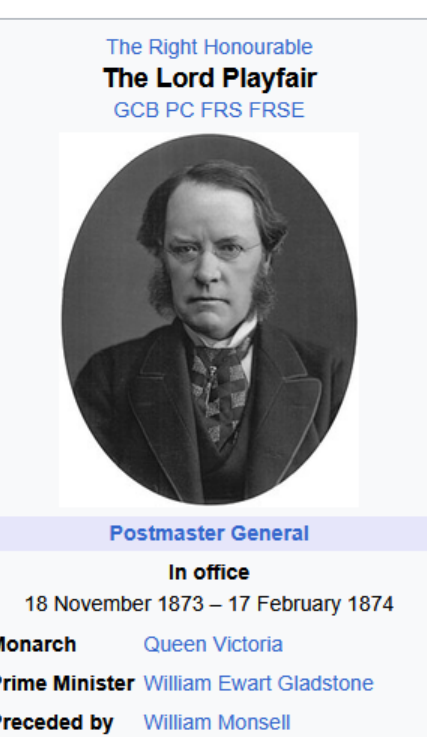
\includegraphics[width=46.62mm,height=204.34mm]{../../images/llm/page_067_img_01.png}%
\end{textblock*}

\end{document}
